\section{XML-Daten- und Dokumentmodelle, XML-Anfragen}

\subsection{Daten- und Dokumentmodelle mit XML}
\begin{itemize}
	\item \textbf{Die Hypertext- und Dokumentwelt vor XML}
	\begin{itemize}
		\item Idee, Struktur zu kennzeichnen führte zu Generalized Markup
		\item 1986 Veröffentlichung von SGML (Standard Generalized Markup Language)
		\item HTML fürs Netz entwickelt\\
		Anwendung von SGML (DTD)\\
		Kompromiss zw. zu viel Komplexität (SGML) und zu wenig Gestaltungsmöglichkeiten (HTML und eingeschränkte Elementtypen)
	\end{itemize}
	
	\item \textbf{Herausforderungen für das WWW}
	\begin{itemize}
		\item Integration der WWW Infrastruktur mit ''echten'' Anwendungen
		\item Zunehmende Professionalisierung
		\item Weiterverwendbarkeit der übertragenen Information auf Benutzerseite
		\item Hohe Anforderungen an das Layout
		\item Metadaten, Zusammenhänge, Sichten
		\item Auffindbarkeit von Information
		\item Verschmelzung mit anderen Medien
	\end{itemize}
	
	\item Warum nicht HTML erweitern?
	\begin{itemize}
		\item keine Erweiterbarkeit durch Benutzer
		\item keine Datenmodellierung
		\item nicht medienneutral
		\item keine clientseitige Verarbeitung {\tiny(was meint er damit?!)}
		\item kein natürliches Navigationskonzept
		\item unnatürliche Aufteilung in ''Seiten''
		\item Nur Volltextsuche mgl
		\item Redundanz; keine strukturelle Integrität
		\item Layoutorientiert, somit kurzlebig
	\end{itemize}
	
	\item \textbf{XML-Entwurfskriterien}
	\begin{itemize}
		\item Unterstützung eines breiten Spektrums von Anwendungen
		\item Modellierung bel. Datentypen
		\item Aufwärtskompatibel zu SGML
		\item nicht voll abwärtskomtabiel zu HTML
		\item einfach genug für Massennutzung
		\item vereinfachtes Parsing durch neues Konzept der Wohlgeformtheit
		\item Minimale Zahl von optionalen MErkmalen
		\item keine semantischen Anteile
		\item Unabhängigkeit von logischer und physikalischer Struktur (''Entitäten'') 
	\end{itemize}
	
	\item \textbf{XML-Dokumentklassen}
	\begin{itemize}
		\item drei Klassen von XML-Dokumenten beschreiben auch die Anwendungsklassen von XML:
		\item \textit{Dokument-zentriert:} tief strukturierte Dokument-Hierarchie für viele Dokumentinstanzen (zb Buch)
		\item \textit{Daten-zentriert:} große Bestände in DBS von dort aus in ein XML-Format generieren Anwendung mit vielen gleichartigen Elementen (DTD ist speziell)\\
		Bsp: EDI (Eletronic Data Interchange): Datenformat zur Kommunikation zw. Anwendungs-/Software-Systemen
		\item \textit{Semi-etrukturiert:} sowohl daten- als auch dokumentzentriert (etwa wissenschaftlicher Artikel)\\
		Merkmale:
		\begin{itemize}
			\item Struktur der Daten ist unregelmäßig und unvollständig
			\item Schema ist implizit in den Daten enthalten
			\item Schema ist flexible, relativ groß, unterliegt häufig Veränderungen
			\item Trennung zw Daten und Schema ist unscharf
		\end{itemize}
	\end{itemize}
	
	\item \textbf{Varianten des XML-Processing}
	\begin{itemize}
		\item Client-basiert:
		\item Quelldaten an Client
		\item Processing Instructions spezifiert Style Sheet
		\item Client übernimmt Bearbeitung
		\item Nachteil: CLient muss XML-Kenntnisse besitzen\\
		\\
		\item Server-basiert:
		\item Client beherrscht XML nicht
		\item Anfrage, welche Formate Client verarbeiten kann
		\item Server schickt Daten zb als HTML
		\item Nachteil: Last auf Server-Seite
	\end{itemize}
	
	\item XML-Technologien im Überblick
	\begin{itemize}
		\item XML: Extensible Markup Language
		\item DTD: Document Type Definition, XML Schema
		\item XSL: Extensible Stylesheet Language, XSLT, XPath, XQUery
		\item XLL: Extensible Linking Language, XLink, XPointer
		\item DOM: Document Object Model, SAX
	\end{itemize}
\end{itemize}

\subsubsection{XML-Dokument}
\begin{itemize}
	\item logische Struktur:\\
	wird durch DTD festgelegt\\
	Deklaration, Elemente, Attribute, Kommentare...
	\item physikalische Struktur\\
	Entities (Makro-, Datei-Include-Mechanismus)\\
	auch nicht-XML-Daten\\
	wiederverwendbar
	
	\begin{figure}[!h]
		\centering
		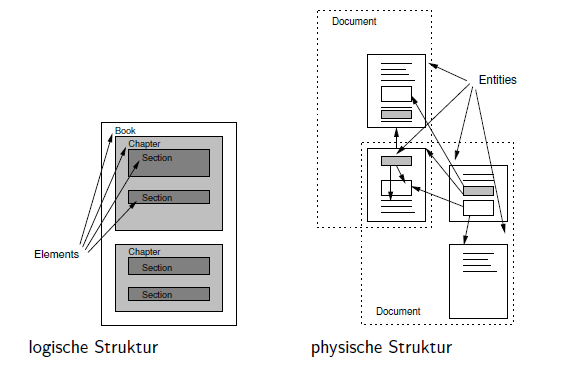
\includegraphics[scale=0.7]{img/xml_structure.png}
	\end{figure}
	
	\item \textbf{Dokument-Aufbau}
	\begin{itemize}
		\item ein oder mehr Elemente <element>,</element>,<element.../>
		\item einfacher Text, \#PCDATA\\
		alle Zeichen in angegebener Kodierung\\
		Zeichen, die Teil des Markups sind mit \&NAME; ersetzen (Entity-Referenzen)
		
		\item für den Text, in dem alle Zeichen erlaubt sind und keine Entity-Referenzen benutzt werden:
		\begin{lstlisting}
		<!CDATA[<markup>
		selbst die Zeichen < und > koennen verwendet werden</markup>]]>
		\end{lstlisting}
		
		\item Elemente können Attribute besitzen, Zuordnung von (default-)Werten mgl
		\item leere (EMTPY) Elemente werden unterstützt, kein Text zwischen den Tags, shortcut: <element.../>
	\end{itemize}
	
	\item \textbf{Processing Instruction}
	\begin{itemize}
		\item Anweisungen für die Verarbeitung des Dokuments durch externe Anwendung
		\item zwischen <? und ?>
		\item keine Einschränkung für Anweisung, außer Zeichenkette ?>
	\end{itemize}
	
	\item \textbf{DTD}
	\begin{itemize}
		\item Regeln wie Elemente, Attribute und andere XML-Daten def. werden
		\item beschreibt strukturellen Aufbau und logische Elemente einer Klasse von Dokumenten
		\item jedes Element, das in XMl-Dokument vorkommt, muss hier def. sein
	\end{itemize}
	\item Markup-Deklaration
	\begin{itemize}
		\item eingeschlossen in <!..>, gruppiert mit <!...[...]>
		\item <!DOCTYPE...>, Dokumenttypfestlgeung
		\item <!--..--> Kommentare
		\item <!ENTITY...> Entity-Deklaration
		\begin{itemize}
			\item <!ENTITY entityname zeichenkette>
			\item Ersetzung von Zeichenketten in XML-Dokuemnten
			\item bestehende Entities für <, >, \&, ' und ''
			\item keine rekursiven Deklaration mgl
		\end{itemize}
		\item <!NOTATION...> Notationstypen
		\item <!ELEMENT...> Elemente
		\begin{itemize}
			\item <!ELEMENT elementname regel>
			\item zw Tags können Zeichenketten stehen
			\item aber auch weitere Elemente
			\item Achtung: kein Elementtyp mehr als einmal deklariert!
			\item Elemente-Subelemente-Hierarchien:\\
			Sequenzen $E (E_1, E_2, \ldots)$\\
			Alternativen $E (E_ \mid, E_2 \mid E_3)$\\
			Quantifizierer $E?, E+, E*$\\
			Gruppierung $E ((E_1, E_2) \mid E_3)$
			
			\item Inhaltsmodelle
			\begin{itemize}
				\item Empty, leere Element wie etwa <p/>\\
				<!ELEMENT E EMPTY>
				\item Element content, Sequenzen, Alternativen, Quantifizierer, Gruppierung\\
				<!ELEMENT E (E$_1$ ...)>
				\item Data content\\
				<!ELEMENT E (\#PCDATA)>
				\item Mixed content, aus volltext und Markup-Element gemischt\\
				<!ELEMENT E (\#PCDATA $\mid$ E$_1$ $\mid$ ...)*>
				\item open content, nur eingeschränkt (ANY), eines der def. Elemente\\
				<!ELEMENT E ANY>
			\end{itemize}
		\end{itemize}
		\item <!ATTLIST...> Attribute zum Element
		\begin{itemize}
			\item <!ATTLIST element attr\_name attr\_typ default\_wert ...>
			\item Definition von Attributen für gegebenen Elementtyp
			\item Typbeschränkungen für Attribute
			\item Vorgabewerte für Attribute
			\item Informationen, ob Attribut vorkomme muss oder wie XML-Prozessor bei fehlendem Attribut reagieren soll
			\item \#REQUIRED, notwenid - Attribut muss immer angegeben werden
			\item \#IMPLIED, impliziert, es gibt keinen Vorgabewert, Prozessor zeigt aber definiertes Verhalten
			\item \#FIXED, fest, alle Instanzen müssen diesen Vorgabewert haben
			\item XML-Attributtypen
			\begin{itemize}
				\item Zeichenkettentyp (CDATA)
				\item Aufzählungstyp (enumerated), Liste von Werten, von denen einer ausgewählt werden muss
				\item Menge von Token-Typen, zb\\
				ID/IDREF eindeutige Identifikation eines Element\\
				ENTITY, in DTD deklarierte Entity kann benutzt werden\\
				NOTATION, Elementinhalt wird abhängig von diesem Attribut interpretiert, muss zuvor mit <!NOTATION> deklarisert sein
			\end{itemize}
		\end{itemize}
		\item <![IGNORE[...]> bedingte Abschnitte
		\item <![INCLUDE[...]> Einfügen von DTD Teilen, Modularisierung
	\end{itemize}
	
	\item \textbf{Wohlgeformte XML-Dokumente}
	\begin{itemize}
		\item DTD benutzen oder in XML-Deklaration Attribut standalone=''no''
		\item Elemente stets öffnendes und schließendes Tag (außer leeres Element)
		\item Element-Tags korrekt geschachtelt
		\item leeres Element schließt mit Zeichenfolge />
		\item \& und < ausschließlich als Markup-Begrenzungen, innerhalb Kommentare, Processing Instructions oder CDATA-Abschnitt
		\item Werte der Attribute in Anführungszeichen
		\item Wohlgeformtheit ohne DTD: alle Attribute vom Typ CDATA
	\end{itemize}
	
	\item gültige XML-Dokumente
	\begin{itemize}
		\item besitzt Dokumenttyp-Deklaration (und hält sich an deren Beschränkungen)
		\item Dokumenttyp steht vor dem ersten Element
		\item enthält oder verweist auf Markup-Deklarationen, Grammatik, DTD
		\item Dokument mit externer DTD: <!DOCTYPE mytpye SYSTEM ''mytype.dtd''>
		\item Dokument mit interner DTD: <!DOCTYPE mytype [...]>
	\end{itemize}
\end{itemize}

\subsubsection{XSL - Style Sheet Language}
\begin{itemize}
	\item Beschreibung wie Elemente angezeigt werden sollen
	\item kann für bel. viele Elemente gelten
	\item für HTML: CSS; für SGML: DSSSL
	\item XSL-Komponenten:\\
	XPath Qualifikation von Dokumentteilen\\
	XSLT ausführende Transformationen\\
	Formating objects fo, allgemeine Formatierungen
	\item Entwurfskriterien
	\begin{itemize}
		\item medienunabhängiges Layoutmodell
		\item Internationalisierung
		\item abwärtskompatibel zu DSSSL; aufwärtskompatibel zu CSS1
		\item regelbasiertes Paradigma:\\
		Regeln bestehen aus zwei Teilen: \textit{template pattern}
		\begin{itemize}
			\item <xsl:template match=''elementname''>
			\item für root-Element auch match=''/''
			\item Menge von Zusätzen zb match=''text/body''
			\item außerdem Reihe von Funktionen, zb first-type-of()
			\item optionale Element vor <xsl:template>, zb <xsl:import>
		\end{itemize}
		und \textit{template action}
		\begin{itemize}
			\item Menge von XSL-Elementen
			\item minimal leeres Element, Regel für alle Kinder des betreffenden Elementtyps
			\begin{figure}[!h]
				\hspace{-7cm}
				\begin{lstlisting}
				<xsl:template match="paragraph">
					<fo:block font-size="18pt">
						<xsl:apply-templates/>
					</fo:block>
				</xsl:template>
				\end{lstlisting}
			\end{figure}
		\end{itemize}
		\begin{itemize}
			\item 
		\end{itemize}
		\item Deklarative und funktionale Sprachanteile, Turing-vollständig
		\item Umstrukturierung der Daten mgl
		\item verwendet selbst XML-Syntax
	\end{itemize}
	\item Designprinzipien
	\begin{itemize}
		\item über Internet einfach nutzbar
		\item deklarative Sprache für normale Formatierungen
		\item Ausweg in Scriptsprache für komplexere Formatierungen, Erweiterbarkeit und Vollständigkeit
		\item Untermenge von DSSSL
		\item Abbildung von CSS in XSL-Style-Sheet soll mgl sein
		\item markups als Formatierungsregeln für Elemente
	\end{itemize}
\end{itemize}

\subsubsection{XML Linking Language (XLink)}
\begin{itemize}
	\item Entwurskriterien
	\begin{itemize}
		\item Links haben Objektcharakter
		\item bidirektionale Links, externe Links
		\item Freie Gestaltung der Ankerelemente
		\item keine reservierten Elementnamen
		\item keine Anfragesprache für Textdatenbanken
		\item geeignet für multimediale Objekte
	\end{itemize}
	
	\item Teilstandards: XLink und XPointer
	\begin{itemize}
		\item beide realisieren zsm die verschiedensten Formen von Hyperlinks
		\item XLink: einfache (ähnlich wie in HTML) und erweiterte (können mit Metadaten annotiert werden) Verweise sind mgl
		\item XPointer: Realisierung von Hyperlinkgs, die nicht nur auf ganze XML-Dokumente zeigen, sondern auf Bestandteile
		Bestandteile werden durch XPath-Ausdrücke angegeben
		\begin{figure}[!h]
			\centering
			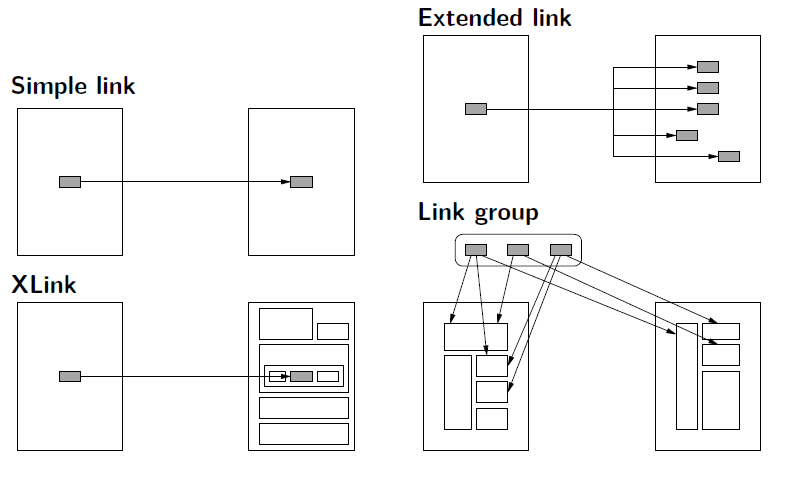
\includegraphics[scale=0.4]{img/hyperlink_types.png}
			\caption{Grundlegende Formen von Hyperlinks}
		\end{figure}
	\end{itemize}
	
	\newpage
	\item Attribut xml:link zeigt an, dass Element ein Verweis ist
	\item kann folgende Werte annehmen: simple - einfacher Link; extended - erweiterter Link
	\item Attribute steuern die Aktivierung:
	\begin{itemize}
		\item xlink:href enthält den eigl Verweis
		\item xlink:role, xlink:arcrole, xlink:title Festlegung Semantik des Linkgs, Verwenden der URIs bzw. textuelle Beschreibung
		\item xlink:show (new|replace|embed|other|none): Anzeige des Verweises wird gesteuert
		\item xlink:actuate (onLoad|onRequest|other|none): Zeitpunkt der Auswertung des Verweises wird festgelegt
	\end{itemize}
\end{itemize}

\subsubsection{DOM}
Entwurskriterien
\begin{itemize}
	\item Trennung von Daten und Programm
	\item Interaktive Dokumente, DB
	\item Inkaufnahme von Systemabhängigkeit
	\item keine Verletzung der Dokumentintegrität darf mgl sein
	\item enge Integration mit Java: JDOM
\end{itemize}


\subsubsection{XML-Anwendungen}
\begin{itemize}
	\item Wissenschaft: Strukturformeln und Messdaten (CML)
	\item Computer, Internet: Push-Kanaäle (CDF); Distribution von Software (OSD); Masken für DB (WIDL)
	\item Workflow, Finanzen: Finanzdaten (OFE), Produktdaten (EDI)
	\item Metadaten, soziale Protokolle: Relationen zw Objekten (RDF); Verteilung von Autoren (WEBDAV)
\end{itemize}

\subsubsection{Zusammenfassung}
\begin{itemize}
	\item Evolutionärer Schritt des WWW
	\item Koexistenz mit HTML und SGML
	\item Öffnet das WWW für Datenaustausch und -verarbeitung
	\item liefert theoretische Grundlagen für neuartige Anwendungen des WWW
	\item Problemorientierung statt WWW-Hacking
	\item WWW soll strukturierter Wissensraum statt lose Blattsammlung werden
\end{itemize}


\subsection{XML-Pfadausdrücke: XPath}